% !TEX root = ../main.tex
\chapter{Le Web sémantique}
\label{annexe:semantic-web}
% TOOD: les ordinateurs et les utilisateurs VS
% ordinateurs et utilisateurs.

% the original text: ``The Semantic Web is an extension of the current
% web in which information is given well-defined meaning, better
% enabling computers and people to work in cooperation.''

L'expression \emph{``Web sémantique''} trouve ces origines dans un
article révolutionnaire publié par Tim Berners-Lee \emph{et
  al.}~\cite{berners2001semantic} en \date{2001}. Le terme fait
d'abord référence à la vision du Web de demain comme un vaste espace
d'échange de ressources entre les êtres humains et les machines
permettant une exploitation, qualitativement supérieure, de grands
volumes d'informations et de services variés. D'après ses promoteurs
\emph{``le Web sémantique est une extension du Web actuel avec une
  signification bien définie des informations. Il permet une meilleur
  coopération et d'échanger l'information entre les ordinateurs et les
  utilisateurs.''}\medskip

Aujourd'hui, le Web Sémantique désigne une infrastructure
technologique visant à rendre le contenu des ressources du Web
accessible et utilisable par des logiciels ou des agents grâce à un
ensemble des langages et des standards initiés et maintenus par le
consortium \acrshort{w3c}. Ces langages sont organisés en couches
d'expressivité croissante permettant l'ajout d'une
\emph{\textbf{``sémantique explicite''}} au contenu des ressources
Web. Cette vision va transforme le Web actuel de documents en Web des
connaissances (ou \emph{Knowledgeable web}~\cite{decker2000semantic}),
ce qui contribue largement au développement de nouvelles approches
plus flexibles pour le partage des données, la réutilisation et
l'intégration de différentes applications.\medskip

%% TODO: éliminer la duplication du terme "Web sémantique"
Dans la suite, nous introduisons la vision globale du Web sémantique,
leur objectifs et principes
fondamentaux~\ref{sec:semantic-web-vision}. Ensuite Nous allons
présenter les principaux standards et langages développés par la
communauté pour la réalisation et la concrétisation du web
sémantique~(\ref{sec:semantic-web-rdf}~\ref{sec:semantic-web-owl}).

\newpage
\section{La vision du Web sémantique}
\label{sec:semantic-web-vision}

%!TEX root = ../../main.tex
\begin{figure}[h]
    \centering
    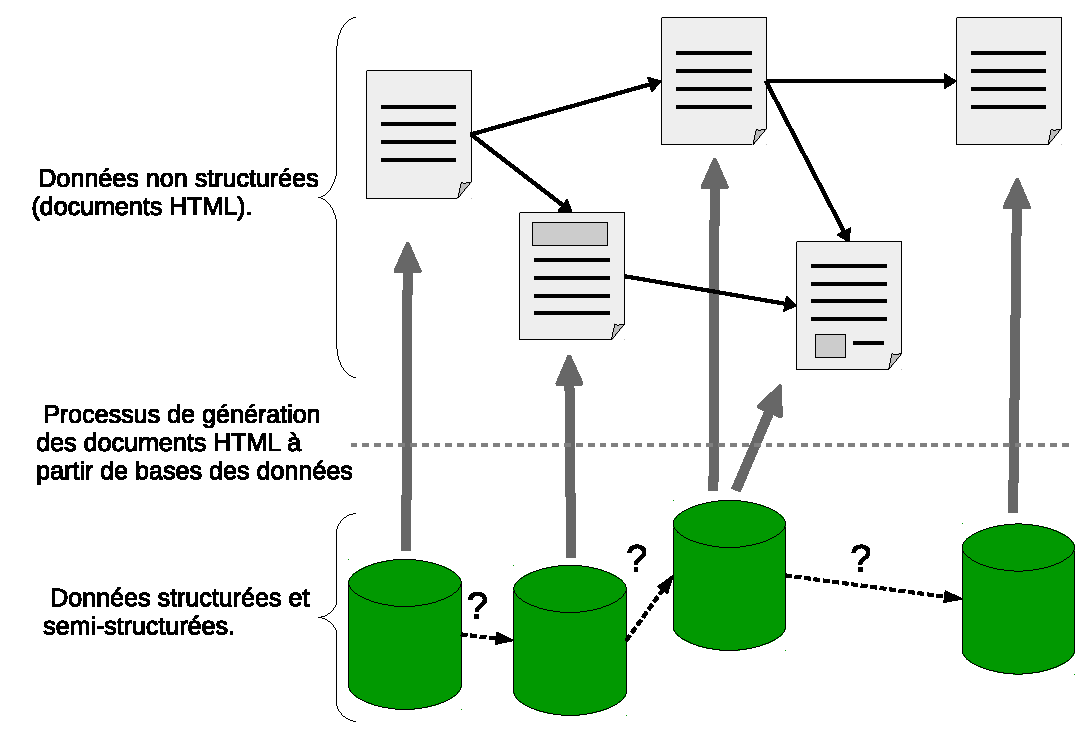
\includegraphics[width=1\textwidth]{figs/A/structured-and-unstructured-data-on-the-web.eps}
    \caption{Les données structurés et non-structurés du
      Web~\cite{antoniou2012semantic}.}\label{fig:structured-and-unstructured-data-on-the-web}
\end{figure}
%%% Local Variables:
%%% mode: latex
%%% TeX-master: "../../main"
%%% End:


Le Web actuel est essentiellement \emph{\textbf{syntaxique}}, dans le
sens que la structure des documents est bien définie mais que son
contenu reste quasi inaccessible aux traitements machines. Il s'agit
d'un Web de documents, les resources sont structurées en
\acrshort{html}, identifiés de manière unique par des \acrshort{uri}
reliés entre eux par des liens hypertextes. L'information est
essentiellement textuelle et la strucure riche qui est généralement
conçus au préalable dans des schémas relationnelles est presque
complètement perdu dans le processus de publication de telles données
sous formes des documents \acrshort{html}. La nouvelle génération de
Web nommée \emph{``Le Web sémantique''} a pour ambition de lever cette
difficulté. Les ressources du Web seront plus aisément accessibles
aussi bien par l'homme que par la machine, grâce à la représentation
\emph{\textbf{sémantique}} de leurs contenus.\medskip

\newpage
\section{La description des ressources Web: RDF}
\label{sec:semantic-web-rdf}
%% Dans cette section on va parler de RDF/RDFS

\section{Langage de définition des ontologies: OWL}
\label{sec:semantic-web-owl}

% What is semantic web?

% Le Web tel que nous le connaissons aujourd'hui est encore conforme à
% la vision initiale.

% Le Web a été conçu principalement pour une utilisation par les
% humains. Néanmoins, il existe un effort visant à automatiser son
% utilisation et d'être plus accessible pour les machines.

% \cite{bartalos2011effective} The Web was primarily designed for use
% by humans. Nevertheless, there is an effort to automate its use and
% bring the Web more accessible for machines. This has brought forward
% the need for machine processable representations of semantically
% rich information. This has brought forward the need for machine
% processable representations of semantically rich information: a
% vision at the heart of the Semantic Web

% Dans un premier temps, on va essayer de clarifier la notion d'un
% service Web sémantique, puis étudier les langages émergeants qui
% permettent de décrire ce type de service Web.

% L'objectif premier du Web sémantique est de définir et lier les
% ressources du Web afin de simplifier leur utilisation, leur
% découverte, leur intégration et leur réutilisation dans le plus
% grand nombre d'applications \cite{berners2001semantic}. Le Web
% sémantique doit fournir l'accès à ces ressources par l'intermédiaire
% de descriptions sémantiques exploitables et compréhensibles par des
% machines. En effet, Les technologies du Web sémantique complètent le
% Web actuel avec des outils sémantiques. Il ne s'agit donc pas de
% créer un nouveau Web ou un Web séparé de l'existant : ce Web de
% données repose entièrement sur les technologies et concepts qui ont
% fait le succès du Web tel que nous le connaissons aujourd'hui
% \cite{bertails2010web}.

% La réalisation du Web sémantique trouve ces racines dans le
% développement des langages de balises inspiré par des travaux issus
% de la communauté AI \cite{mcilraith2001semantic}, tels que
% \textsc{OIL} \cite{fensel2001oil}, \textsc{DAML+OIL}
% \cite{horrocks2002daml+oil} et \textsc{DAML+OTN}
% \cite{mcguinness2003daml} (ces deux derniers langages font partie de
% la famille \acrshort{daml}).

% TODO refactor Ces langages ont une sémantique bien définies et
% permettent le balisage et la manipulation des taxonomies complexe et
% des relations logiques entre les entités sur le
% Web. \cite{fensel2000creating}

% \input{figs/3w_to_sws.tex}

% Cette description repose sur des ontologies. Selon Gruber
% \cite{gruber1993translation}, une ontologie est une spécification
% explicite d'une conceptualisation. Une conceptualisation est un
% modèle abstrait qui représente la manière dont les personnes
% conçoivent les choses réelles dans le monde et une spécification
% explicite signifie que les concepts et les relations d'un modèle
% abstrait reçoivent des noms et des définitions explicites. Le Web
% sémantique est devenu un domaine à part entière, preuve en est la
% création en 2001 du groupe de travail sur ce sujet par le
% \textsc{W3C}.

%%% Local Variables:
%%% mode: latex
%%% TeX-master: "../main"
%%% End:
